\documentclass[11pt]{article}
\usepackage{tikz}
\usetikzlibrary{positioning,fit,backgrounds}
\usepackage[normalem]{ulem}
\usepackage{cs1200}

\begin{document}

\psHeader{8}{Wed Nov. 12, 2025 (11:59pm)}

Please see the syllabus for the full collaboration and generative AI policy, as well as information on grading, late days, and revisions.

All sources of ideas, including (but not restricted to) any collaborators, AI tools, people outside of the course, websites, ARC tutors, and textbooks other than Hesterberg--Vadhan must be listed on your submitted homework along with a brief description of how they influenced your work. You need not cite core course resources, which are lectures, the Hesterberg--Vadhan textbook, sections, SREs, problem sets and solutions sets from earlier in the semester. If you use any concepts, terminology, or problem-solving approaches not covered in the course material by that point in the semester, you must describe the source of that idea. If you credit an AI tool for a particular idea, then you should also provide a primary source that corroborates it. Github Copilot and similar tools should be turned off when working on programming assignments.

If you did not have any collaborators or external resources, please write 'none.' Please remember to select pages when you submit on Gradescope. A problem set on the border between two letter grades cannot be rounded up if pages are not selected.

\vspace{1em}

\textbf{Your name: }

\textbf{Collaborators and External Resources: }

\textbf{No. of late days used on previous psets: }

\textbf{No. of late days used after including this pset: }

\vspace{1em}

The purpose of this problem set is to develop skills in implementing graph algorithms, appreciate the impact of different kinds of worst-case exponential algorithms in practice, and practice reducing problems to SAT.
\begin{enumerate}


\item (Another coloring algorithm) 
  In the Github repository for PS8, we have given you basic data structures for graphs (in adjacency list representation) and colorings, an implementation of the coloring algorithm from ps6, and a variety of test cases (graphs) for coloring algorithms. 


  
  \begin{enumerate}
      
      \item Implement the reduction from 3-coloring to SAT given in class in the function \texttt{sat\_3\_coloring}, producing an input that can be fed into the SAT Solver \href{https://pysathq.github.io/usage/}{Glucose}, and verify its correctness by running \texttt{python3 -m ps8\_tests 3}. \label{part:SAT}
     

    
      

  

    
      \item Compare the efficiency of Exhaustive-Search 3-coloring, the $O(1.45^n)$-time independent-set and BFS algorithm for 3-coloring from problem set 6 (feel free to use the staff solution or your own implementations from problem set 6), and your implementation from  Part~\ref{part:SAT} using \texttt{ps8\_experiments}. In the experiments file, we've provided code to generate two types of graphs (lines of rings and clusters of independent sets) and some new hard graph instances. For each of those types of graphs, how many of the given instances, if any, can each algorithm solve within 1 second? You should fill out the table and briefly discuss your findings, as well as why these algorithms perform the way they do given what we have discussed in lecture.
    

\begin{center}
    \begin{tabular}{|c|l|l|l|}
    \hline 
    Algorithm
    & \multicolumn{1}{|p{2cm}|}{Exhaustive}
    & \multicolumn{1}{|p{2cm}|}{ISET BFS}
    & \multicolumn{1}{|p{2cm}|}{SAT Color}\\\hline
    \hline
        \# Solvable Ring Instances &  &  & \\
        \# Solvable Cluster Instances  &   & &  \\
        \# Solvable Hard Graphs  &   & &  \\
        \hline
    \end{tabular}
\end{center}

      


  \end{enumerate}

\item (Resolution) Use the algorithm \texttt{ResolutionInOrder} (algorithm 18.2 from the textbook) to decide the satisfiability of the following formulas, and use the algorithm \texttt{ExtractAssignment} to obtain a satisfying assignment for any that are satisfiable. (Please make sure to follow both algorithms \textit{exactly}, including the order in which the clauses are processed. A correct final solution that does not show all of the intermediate steps of both algorithms will not receive full score.)



  
  \begin{enumerate}
      

 \item $\varphi(x_0, x_1, x_2, x_3) = (x_0) \wedge (x_2 \vee x_3)\wedge ( x_1 \vee  x_2)\wedge ( x_1 \vee  x_0)$\


 
  \item $\varphi(x_0, x_1, x_2, x_3) = (\neg x_1) \wedge ( x_3) \wedge (\neg x_2 \vee \neg x_3)\wedge ( x_1 \vee  x_2)$
 

 
  

 \item $\varphi(x_0, x_1, x_2, x_3) = (\neg x_1 \vee \neg x_2) \wedge (x_3 \vee x_1) \wedge (\neg x_0 \vee x_3) \wedge (\neg x_3) \wedge ( x_0 \vee \neg x_1)$


  \item $\varphi(x_0, x_1, x_2, x_3, x_4) =  ( x_1 \vee  \neg x_2 \vee x_3\vee \neg x_4)\wedge ( x_0 \vee  x_4) \wedge ( \neg x_2 \vee  x_4)\wedge ( x_3 \vee  x_0)\wedge (\neg x_3 \vee  x_4)$



  \end{enumerate}

  

\item (Reductions to SAT) In Section 15.3 of the textbook, we saw an efficient algorithm to solve the Maximum Matching problem in Bipartite Graphs. A variant of Maximum Matching is Maximum 3-D Matching, where we are given not a graph $G=(V,E)$ but a ``3-uniform hypergraph'' $H=(V,E)$, where the {\em hyperedges} $e\in E$ now are {\em triples} of vertices.  
Analogously to restricting to bipartite graphs, we restrict to {\em tripartite} hypergraphs where $V$ is the union of 3 disjoint sets $V_0\cup V_1 \cup V_2$ and every hyperedge $e\in E$ has exactly one vertex from each of $V_0,V_1,V_2$. For example, hyperedges may consist of 
compatible patient-donor-timeslot triples (if there are only certain timeslots in which a patient and donor are available for a surgery), 
or compatible surfer-surfboard-fins triples (if each surfer only likes to ride certain surfboards with certain fins installed).
Now the goal is to find a maximum-sized set $M\subseteq E$ such that every vertex $v\in V$ is contained in at most one edge of $M$.  
Unfortunately, unlike matching in graphs, there is no polynomial-time algorithm known for Maximum 3-D Matching, even if we restrict to tripartite hypergraphs and even if we only want to find {\em complete matchings} --- ones that match every vertex in $V_0$ (i.e. we are looking for a matching of size $|M|=|V_0|$):
\compprob{3dCompleteMatching()}
{Three disjoint finite sets of vertices $V_0,V_1,V_2$ and a set $E$ of hyperedges  such that each $e\in E$ contains exactly one vertex from each of $V_0$, $V_1$, and $V_2$.}
{A set $M$ of hyperedges such that every vertex is in at most one hyperedge in $M$, and every vertex in $V_0$ is in a hyperedge in $M$ (if one exists).
}

% picture
\begin{figure}[h]
\centering
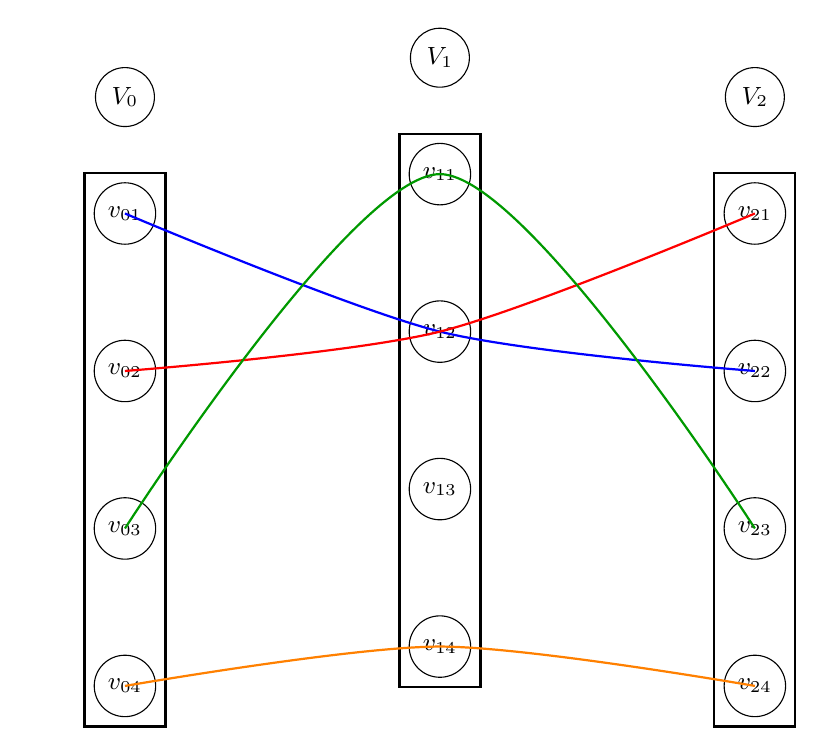
\begin{tikzpicture}[
  every node/.style={circle, draw, minimum size=7mm, font=\small},
  edge/.style={thick, bend left=15}
]

\node (v01) at (0,3) {$v_{01}$};
\node (v02) at (0,1) {$v_{02}$};
\node (v03) at (0,-1) {$v_{03}$};
\node (v04) at (0,-3) {$v_{04}$};

\node (v11) at (4,3.5) {$v_{11}$};
\node (v12) at (4,1.5) {$v_{12}$};
\node (v13) at (4,-0.5) {$v_{13}$};
\node (v14) at (4,-2.5) {$v_{14}$};

\node (v21) at (8,3) {$v_{21}$};
\node (v22) at (8,1) {$v_{22}$};
\node (v23) at (8,-1) {$v_{23}$};
\node (v24) at (8,-3) {$v_{24}$};

\node[above=0.7cm of v01] {$V_0$};
\node[above=0.7cm of v11] {$V_1$};
\node[above=0.7cm of v21] {$V_2$};

\begin{pgfonlayer}{background}
  \node[draw, thick, shape=rectangle, fit=(v01) (v02) (v03) (v04), label=left:{}] {};
  \node[draw, thick, shape=rectangle, fit=(v11) (v12) (v13) (v14), label=left:{}] {};
  \node[draw, thick, shape=rectangle, fit=(v21) (v22) (v23) (v24), label=left:{}] {};
\end{pgfonlayer}

\draw[thick, color=blue, smooth]
  plot coordinates {(v01) (v12) (v22)};

\draw[thick, color=red, smooth]
  plot coordinates {(v02) (v12) (v21)};

\draw[thick, color=green!60!black, smooth]
  plot coordinates {(v03) (v11) (v23)};

\draw[thick, color=orange, smooth]
  plot coordinates {(v04) (v14) (v24)};

\end{tikzpicture}

\caption{\centering Example of hypergraph with sets of vertices $V_0 = [v_{01}, v_{02}, v_{03}, v_{04}], V_1 = [v_{11}, v_{12}, v_{13}, v_{14}], V_2 = [v_{21}, v_{22}, v_{23}, v_{24}]$ and hyperedges $E = \{(v_{01}, v_{12}, v_{22}), (v_{02}, v_{12}, v_{21}), (v_{03}, v_{11}, v_{23}), (v_{04}, v_{14}, v_{24})\}$}



\end{figure}

\newpage
\begin{enumerate}
\item Show that there is a polynomial-time reduction of 3dCompleteMatching to SAT that, on hypergraphs with $n=|V_0|+|V_1|+|V_2|$ vertices and $m=|E|$ hyperedges, makes one oracle query on a formula with $m$ variables and $O(n + m^2)$ clauses, and runs in time $O(n + m^2)$.  Be sure to prove the correctness of your algorithm and analyze its runtime. 

Optionally, justify why the reduction can be implemented in time $O(m^2)$ (this can be part of an attempt at an R+ on this problem, but is not required for full credit). Thus, even though the fastest known algorithms for 3dCompleteMatching run in exponential time, we can use SAT Solvers to solve it much more efficiently on many instances that arise in practice. 






\fi

\item (optional\footnote{This problem won't make a difference between N, L, R-, and R grades. As this problem is purely extra credit, course staff will deprioritize questions about this problem at office hours and on Ed.}) Come up with a polynomial-time reduction for the version of 3dMatching where we are also given a number $k\in \N$ as part of the input and want to find a matching of size $k$ (rather than one of size $|V_0|$).  (Hint: you will probably want to use more than $m$ boolean variables, at least $k\cdot m$, possibly more, depending on how you approach the problem.)




\end{enumerate}


\item (reflection) \textbf{Active learning} involves engaging in activities that require you to think critically and apply your knowledge. Examples of active learning include reading the textbook carefully, asking questions, solving practice problems, and teaching concepts to others. In contrast, \textbf{passive learning} refers to taking in information without actively engaging with it--for instance, watching a lecture without participating, or listening to a collaborator or AI explain course concepts to you. Active learning has been shown to be more effective than passive learning for developing a deep understanding of course material.

In CS 1200, which active learning strategies do you use? Are there passive learning habits you tend to rely on? Reflect on your current approach: Are you satisfied with the amount of active learning you're incorporating? Why or why not? If you think you could benefit from more active learning, what specific steps could you take to engage more actively in CS 1200?

Quick note on grading: Good responses are usually about a paragraph, with something like 7 or 8 sentences. Most importantly, please make sure your answer is specific to this class and your experiences in it. If your answer could have been edited lightly to apply to another class at Harvard, points will be taken off.

\item Once you're done with this problem set, please fill out \href{https://docs.google.com/forms/d/e/1FAIpQLSdxPDzaj-5cIolKoLC15s3Jd-rp1C-zDCdipmD3u4H23-y5BQ/viewform?usp=sharing&ouid=102370254274488295019}{this survey} so that we can gather students' thoughts on the problem set, and the class in general. It's not required, but we really appreciate all responses!

\end{enumerate}

\end{document}
